\section{Certified basins of attraction}\label{sec:certificates}

The critical kick $\Delta v^*$ of Section~\ref{sec:bistability} samples the basin of the forced orbit in one direction of the state space, at 16 phases and on a grid of kick sizes; it cannot exclude chatter after a disturbance in another direction. This section proves inner estimates of the basin instead: ellipsoids of deviations from the forced orbit from which every trajectory returns to the orbit despite the clip. Unlike regional guarantees for chatter controllers designed with input constraints \citep{zhang2015ellipsoid,wu2016adaptive}, the DVF law is fixed and analysed, the clip acts on the voltage, and the dead zone is taken around the forced command $b(t)$, so that the authority spent on the forced orbit enters the certificate. Certificate C2 uses the averaged model and C3 the time-periodic model; both are checked independently of the solver and compared with the simulator of \ref{app:simulator}.

\subsection{Deviation dynamics and what is proved}\label{sec:cert-model}

Let $x_p(t)$ be the $T$-periodic forced orbit of Section~\ref{sec:model-orbit} and $b(t)=-g\dot x_p(t)$ its command, with $\bmax<\Vmax$ so that the clip is inactive on the orbit. Since $x_p(t)-x_p(t-T)=0$, the regenerative force vanishes on the orbit, and the deviation $\tilde x=x-x_p$ obeys
\begin{equation}\label{eq:dev}
\begin{aligned}
&m\ddot{\tilde x}+c\dot{\tilde x}+k\tilde x=aH(t)\,\big[\tilde x(t)-\tilde x(t-T)\big]+K_a\ddot{\tilde q},\\
&\ddot{\tilde q}+2\zeta_a\omega_a\dot{\tilde q}+\omega_a^2\tilde q=\sat_{\Vmax}\!\big(b(t)-g\dot{\tilde x}\big)-b(t),
\end{aligned}
\end{equation}
where $\tilde q$ is the deviation of the actuator coordinate of Eq.~\eqref{eq:eom} and $aH(t)$ is the $T$-periodic coefficient of the regenerative force, Eq.~\eqref{eq:aHt}. C2 replaces it by its mean $\overline{aH}$, Eq.~\eqref{eq:aHmean}, as in the zero-order approximation \citep{altintas1995analytical}; C3 keeps $aH(t)$.

The history $\tilde x(t+\vartheta)$, $\vartheta\in[-T,0]$, is represented by its values at the Chebyshev nodes $\vartheta_j=-\tfrac T2\big(1-\cos\tfrac{\pi j}{N}\big)$, $j=1,\dots,N$, and its transport equation is collocated with the Chebyshev differentiation matrix \citep{breda2005pseudospectral,breda2015book}. With $\xi=\big[\tilde x,\ \dot{\tilde x},\ \tilde q,\ \dot{\tilde q},\ \tilde x(t+\vartheta_1),\dots,\tilde x(t+\vartheta_N)\big]^\top\in\mathbb R^{4+N}$,
\begin{equation}\label{eq:coll}
\dot\xi=\mathcal A(t)\,\xi-B\,\psi(K\xi,t),\qquad \mathcal A(t)=A_0+BK+aH(t)\,E,
\end{equation}
with $K=-g\,e_2^\top$, $E=\big(e_2e_1^\top-e_2e_{4+N}^\top\big)/m$, $e_i$ the unit vectors, and $A_0$, $B$ in Eq.~\eqref{eq:app-A0}. The linear DVF loop stays in $\mathcal A$; the clip enters only through the dead zone
\begin{equation}\label{eq:deadzone}
\psi(w,t)=w-\sat_{\Vmax}\!\big(b(t)+w\big)+b(t),
\end{equation}
which vanishes for $-\Vmax-b(t)\le w\le\Vmax-b(t)$; unlike the dead zone of a fixed saturation, it moves with the forced command and is asymmetric whenever $b(t)\neq0$. The number of nodes is $N=16+4\lceil T\omega_n/2\pi\rceil$, 20--32 over 500--\SI{3000}{\rpm} (24 at 1090 and \SI{1420}{\rpm}, 20 at 2500 and \SI{2870}{\rpm}). For the averaged model the rightmost eigenvalues of Eq.~\eqref{eq:coll} agree with those of the delay equation to $3\times10^{-8}$, and the collocated model loses stability at $\alim$.
% src: README §12.2; src/c2_certificate.py (model, nodes_for, history_nodes); src/c3_periodic.py (model); tests/test_c2_certificate.py (crossing at a_lim)

The certificates are therefore theorems about Eq.~\eqref{eq:coll}, the $N$-node collocation of the averaged (C2) or the time-periodic (C3) model; they are not theorems about the delay equation, which would require a Lyapunov--Krasovskii functional \citep{seuret2014bessel}, nor about the simulator. Two effects of the simulator lie outside Eq.~\eqref{eq:coll}: the chip vanishing near the exit angle and, for C2, the variation of $aH(t)$, about $\pm12\,\%$ around its mean near the limit at half immersion and more at shallow depths.
% src: README §12.2, §14.10

\subsection{Sector condition and LMI conditions}\label{sec:cert-lmi}

Here $\bmax$ denotes an upper bound of $\max_t\lvert b(t)\rvert$, not a sampled peak, and $u_0=\Vmax-\bmax>0$. For all $t$, $w$ and $v$,
\begin{equation}\label{eq:sector}
\lvert w-v\rvert\le u_0\quad\Longrightarrow\quad\psi(w,t)\,\big[\psi(w,t)-v\big]\le0 .
\end{equation}
If $w>\Vmax-b(t)$, then $\psi=w-\Vmax+b(t)>0$ and $v\ge w-u_0\ge\psi$ since $b(t)\le\bmax$; the case $w<-\Vmax-b(t)$ is symmetric, and $\psi=0$ otherwise. Eq.~\eqref{eq:sector} is the generalised sector condition of \citet{gomesdasilva2005antiwindup} for the moving dead zone, with the level $u_0=\SI{9}{\volt}-\bmax$: the authority spent on the forced orbit is removed from the level. With $v=\Gamma\xi$ for a free row vector $\Gamma$, $\mathcal V(\xi)=\xi^\top P\xi$, $W=P^{-1}$, $Y=\Gamma W$ and a scalar multiplier $S>0$, the S-procedure \citep{tarbouriech2011book} gives, for the averaged model ($\mathcal A$ constant),
\begin{gather}
\begin{bmatrix}-(\mathcal AW+W\mathcal A^\top)-2\lambda W & BS-Y^\top\\ SB^\top-Y & 2S\end{bmatrix}\succ0, \label{eq:lmi-dec}\\
\begin{bmatrix}W & WK^\top-Y^\top\\ KW-Y & u_0^2\end{bmatrix}\succeq0, \label{eq:lmi-incl}\\
\begin{bmatrix}W & Wc^\top\\ cW & (\delta f_z)^2\end{bmatrix}\succeq0,\qquad c=e_1^\top-e_{4+N}^\top,\quad \delta=0.5, \label{eq:lmi-valid}\\
\begin{bmatrix}1 & \beta e^\top\\ \beta e & W\end{bmatrix}\succeq0. \label{eq:lmi-size}
\end{gather}
Inequality~\eqref{eq:lmi-incl} places $\mathcal E(P)$ in the region $\lvert(K-\Gamma)\xi\rvert\le u_0$, where Eq.~\eqref{eq:sector} holds with $w=K\xi$, and Eq.~\eqref{eq:lmi-dec} with $\lambda=0$ then makes $\mathcal V$ decrease strictly along every trajectory in $\mathcal E(P)$, at every $t$, because Eq.~\eqref{eq:sector} holds uniformly in time. $\mathcal E(P)$ is thus forward invariant, and every deviation in it returns to the forced orbit, whatever its phase. The margin $\lambda>0$ is asked of the solver only; the independent check tests $\lambda=0$, so no decay rate is claimed.

Inequality~\eqref{eq:lmi-valid} keeps $\mathcal E(P)$, and with it the whole trajectory, inside $\lvert x-x(t-T)\rvert\le0.5f_z$ (as $x_p$ is $T$-periodic, $\tilde x-\tilde x(t-T)=x-x(t-T)$). Without it, the ellipsoid at \SI{2500}{\rpm} and $0.7\alim$ contained states whose past was displaced by 7--12$f_z$, the tool being entirely out of the cut; they return in the linear model, but 32 of the 72 off-axis runs at that point (Section~\ref{sec:cert-c2}) ended in chatter, against 0 of 72 with the bound, whose cost along the kick direction is 0--16\,\%. The bound excludes only gross loss of contact: the chip can still vanish near the exit angle inside it. The value $\delta=0.5$ is a choice; $\delta=1$ raises the certificates by 0--15\,\%.
% src: README §12.2, §12.4, §12.7

The size $\beta$ in Eq.~\eqref{eq:lmi-size} is maximised along two directions. For $e=e_2$, a velocity kick at any phase moves the state to $\Delta v\,e_2$, since displacement and history are continuous, so $\beta$ is a certified kick in m/s. For $e=-\xi_p(0)$, minus the orbit state at $t=0$ with its history, $\beta$ is dimensionless: the cut that enters at rest on a fresh surface starts at $-\xi_p(0)$, so $\beta\ge1$ certifies the step entry at the entry phase of the simulator (tooth angle 0 at $t=0$), and only at that phase.

In C2, $\bmax$ was computed from samples of the orbit truncated at 40 harmonics, whose slice-force coefficients came from a discrete Fourier transform (\ref{app:lmi}). The closed-form bound of C3 is higher by 0.4--\SI{2.1}{\milli\volt} at the 48 validation points and by 0.1--\SI{3.3}{\milli\volt} on the surface grid. As all LMIs are homogeneous in $(W,Y,S)$, a certificate at the level $u_0$ remains valid at $u_0-d$ after scaling $(W,Y,S)$ by $\big((u_0-d)/u_0\big)^2$, which scales its size by $(u_0-d)/u_0$: by 0.997--1.000 at the 48 points and by down to 0.86 on the surface, where the margin almost vanishes. All C2 results below are corrected in this way.
% src: README §12.2, §14.9; results/c3_summary.json (errata: extra_mV 0.414-2.079 and 0.131-3.275, size_factor 0.9972-0.99995 and 0.858-1); src/c3_summary.py (margin_errata)

\subsection{Solution and independent check}\label{sec:cert-check}

The LMIs were assembled as sparse conic programs for the interior-point solver Clarabel \citep{goulart2024clarabel}, which stops short of the optimum on these problems. Each problem was solved three times: in coordinates scaled by the peak response of each state to a \SI{1}{\milli\metre\per\second} kick, then twice in coordinates whitened by the previous $W$ (re-centring). Every candidate $(W,Y,S)$ was checked independently of the solver: (i) $W\succ0$ with a condition number below $10^{10}$; (ii) the smallest eigenvalue of the matrix of Eq.~\eqref{eq:lmi-dec} at $\lambda=0$ above a round-off bound; (iii) the inclusion~\eqref{eq:lmi-incl} and the validity bound~\eqref{eq:lmi-valid}, evaluated through a Cholesky factor of $W$, an exceeded bound being repaired by scaling $(W,Y,S)$ down, which preserves (ii) by homogeneity; (iv) the size $\beta=(e^\top W^{-1}e)^{-1/2}$ from the same factor. The largest candidate that passed was kept, and the smaller of its checked size and the solver's $\beta$ is reported (settings in \ref{app:lmi}).
% src: src/c2_certificate.py (scaling, lmi, check, certify); README §12.3

\subsection{Extension to the time-periodic model}\label{sec:cert-periodic}

C3 keeps the periodic coefficient $aH(t)$ of Eq.~\eqref{eq:aHt}, with the integral over the depth evaluated in closed form. The forced orbit is that of C2, since regeneration vanishes on every $T$-periodic motion. At \SI{2500}{\rpm}, $aH(t)$ spans 0.89--1.08 times its mean at $0.9\alim$ and 0.36--1.42 times at $0.15\alim$, and the forced command $\lvert b(t)\rvert$ ranges over the period from nearly zero to \SI{7.9}{\volt} at $0.98\alim$, whereas C2 uses only its peak.
% src: README §14.1; src/c3_periodic.py (aH, orbit); ranges re-evaluated in closed form with c3_periodic.aH/orbit (0.886-1.079, 0.358-1.420; |b| 0.031-7.870 V)

The tooth period is divided into $M=16$ segments of length $\tau=T/M$, with nodes $t_k=k\tau$. On segment $k$, with $s=(t-t_k)/\tau\in[0,1]$,
\begin{equation}\label{eq:Wt}
W(t)=(1-s)W_k+sW_{k+1},\qquad Y(t)=(1-s)Y_k+sY_{k+1},\qquad S(t)=S_k,
\end{equation}
with $W_M=W_0$ and $Y_M=Y_0$, so that $\mathcal V(t,\xi)=\xi^\top W(t)^{-1}\xi$ is continuous and $T$-periodic. As $\mathrm d(W^{-1})/\mathrm dt=-W^{-1}\dot WW^{-1}$, the decrease condition becomes
\begin{equation}\label{eq:lmi-per}
\begin{bmatrix}\dot W_k-\mathcal A(t)W(t)-W(t)\mathcal A(t)^\top-2\lambda W(t) & BS_k-Y(t)^\top\\ S_kB^\top-Y(t) & 2S_k\end{bmatrix}\succ0,
\end{equation}
with $\dot W_k=(W_{k+1}-W_k)/\tau$, required at every $t$ of the segment. On each segment the coefficient is enclosed as $aH(t)=h_k+\ell_ks+r$, $\lvert r\rvert\le\varepsilon_k$: a least-squares line through 2048 samples and a residual bound widened by the variation possible between samples. $\mathcal A(t)W(t)$ then contains $s$, $s^2$ and $rs$, so that Eq.~\eqref{eq:lmi-per} is affine in $(s,\sigma)$, $\sigma=s^2$, for fixed $r$ and affine in $r$ for fixed $(s,\sigma)$. Since $(s,s^2)$ lies in the triangle with vertices $(0,0)$, $(\tfrac12,0)$ and $(1,1)$, the matrix at any time of the segment is a convex combination of its values at these three points combined with $r=\pm\varepsilon_k$, and positivity at the six vertices gives Eq.~\eqref{eq:lmi-per} on the whole segment.

The sector condition holds pointwise in time, so segment $k$ uses its own level $u_{0,k}=\Vmax-\max_{t_k\le t\le t_{k+1}}\lvert b(t)\rvert$ rather than $\Vmax-\bmax$. Inequalities~\eqref{eq:lmi-incl}--\eqref{eq:lmi-size}, written with $W(t)$, $Y(t)$ and $u_{0,k}$, are affine in $s$ and are imposed at both nodes of each segment. The tube $\{(t,\xi):\xi^\top W(t)^{-1}\xi\le1\}$ is then forward invariant and $\mathcal V$ decreases strictly in it: a deviation in $\mathcal E\big(W(t_0)^{-1}\big)$ at the phase $t_0$ returns to the orbit. As Eq.~\eqref{eq:lmi-size} is affine in $W$, a size that holds at both nodes of a segment holds between them; the certified kick valid at every phase is thus the smallest nodal size, and the sizes at the 16 kick phases of Section~\ref{sec:bistability} follow from $W(t)$ by interpolation. The tools are established, from piecewise-linear or clock-dependent time-varying Lyapunov matrices for switched, impulsive and periodic systems \citep{allerhand2011robust,briat2013clock,li2015periodic} to regions of attraction of saturated periodic systems \citep{zhou2011periodic,yang2015periodic,sakthivel2022jdsmc} and the control of periodic piecewise vibration systems with actuator saturation \citep{li2017hinfinity}, and \citet{cao2020switched} used a piecewise Lyapunov function, without a region of attraction, for active chatter control on a switched periodic milling model; what is new here is the application. The first solve starts in the coordinates of the C2 certificate, and every candidate is checked at all $6\times16$ vertices and all nodes (\ref{app:lmi}).
% src: README §14.2, §14.3, §14.9; src/c3_periodic.py (enclosure, corners, orbit, lmi, check, certify)

\subsection{Results on the averaged model (C2)}\label{sec:cert-c2}

C2 was computed at the 48 clipped points of Section~\ref{sec:bistability} (1090, 1420, 2500 and \SI{2870}{\rpm}; 12 depths from 0.15 to $0.98\alim$; $g=\SI{1500}{\volt\second\per\metre}$; Fig.~\ref{fig:cert}, Table~\ref{tab:cert}). All 48 certificates passed the check, with certified kicks of 0.96--\SI{12.9}{\milli\metre\per\second}. Each lies below the critical kick of its own model (the averaged collocated model with the true dead zone, minimum over four phases) at all 44 points where that kick is finite, and below $\Delta v^*$ (minimum over 16 phases) at all 29 points where $\Delta v^*$ is finite. $\Delta v^*/\beta$ is 1.48--27.6, largest at \SI{2500}{\rpm} and $0.4\alim$ ($\beta=\SI{0.96}{\milli\metre\per\second}$), and 1.48--3.26 (median 2.34) from $0.7\alim$ upwards. The averaged model is slightly more fragile than the simulated cut (critical kick 0.62--0.99 times $\Delta v^*$, median 0.92), so the gap lies mainly between the certificate and its own model.
% src: README §12.4; results/c2_validate.npz, c2_summary.json (validate), c3_summary.json (errata.c2_validate: 1.48-27.59, median 2.34 from 0.7 a_lim)

\begin{figure}[!tbp]
\centering
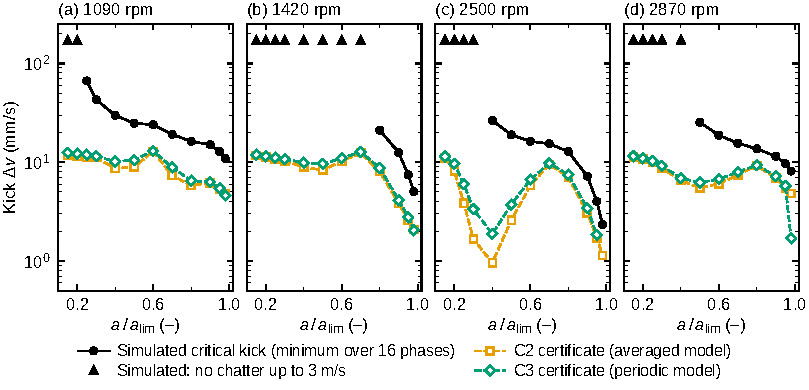
\includegraphics[width=\textwidth]{figures/fig06_certificates.pdf}
\caption{Certified kick on the averaged model (C2, squares; command bound corrected as in Section~\ref{sec:cert-lmi}) and on the periodic model (C3, diamonds; valid at every phase) against the simulated critical kick $\Delta v^*$ (circles; minimum over 16 phases), at (a) 1090, (b) 1420, (c) 2500 and (d) \SI{2870}{\rpm}, $g=\SI{1500}{\volt\second\per\metre}$, $\Vmax=\SI{9}{\volt}$. Triangles: no chatter for any kick up to \SI{3}{\metre\per\second}. C3 is missing at \SI{2500}{\rpm} and $0.98\alim$, where no candidate passed the check. Wherever $\Delta v^*$ is finite, both certificates lie below it.}
\label{fig:cert}
\end{figure}

\begin{table}[!tbp]
\centering
\caption{Validation of the certificates at the 48 clipped points of Section~\ref{sec:bistability} (four speeds, 12 depths from 0.15 to $0.98\alim$, $g=\SI{1500}{\volt\second\per\metre}$). $\Delta v^*$: simulated critical kick; C2 corrected for the command bound.}
\label{tab:cert}
\small
\begin{tabular}{@{}>{\raggedright\arraybackslash}p{0.36\textwidth}>{\raggedright\arraybackslash}p{0.27\textwidth}>{\raggedright\arraybackslash}p{0.27\textwidth}@{}}
\toprule
 & C2 (averaged model) & C3 (periodic model, $M=16$)\\
\midrule
Certificates that passed the check & 48/48 & 47/48\\
Certified kick $\beta$ (\si{\milli\metre\per\second}) & 0.96--12.9 & 1.70--13.0\\
$\beta$ below the model's critical kick & 44/44 (minimum over 4 phases) & 688/688 (per phase, 43 points)\\
$\beta$ below $\Delta v^*$ & 29/29 (minimum over 16 phases) & 448/448 (per phase, 28 points)\\
$\Delta v^*/\beta$, all points & 1.48--27.6 & 1.46--14.0\\
$\Delta v^*/\beta$ from $0.7\alim$ (median) & 1.48--3.26 (2.34) & 1.46--4.78 (2.27)\\
Model critical kick$/\Delta v^*$ (median) & 0.62--0.99 (0.92) & 0.61--0.98 (0.90)\\
Off-axis runs ending in chatter & 0/3456 & 0/3384\\
Sampled check, largest $\mathcal V$ & 0.998 (start value) & 0.997 (after the first step)\\
C3/C2 (median) & -- & 0.35--2.01 (1.064)\\
\bottomrule
\end{tabular}
\end{table}
% src: results/c2_summary.json, c3_summary.json (basin: cert_mm_s, phase_cert_below_model/td, td_over_cert, td_over_cert_from_07, model_over_td, offaxis, proof_vmax, c3_over_c2; errata.c2_validate); results/c2_validate.npz (C2 beta corrected 0.958-12.889 mm/s, model/TD 0.620-0.989)

A kick probes one of $4+N$ directions. Boundary points of $\mathcal E(P)$ in 18 directions (both signs of the points that maximise $\tilde x$, $\dot{\tilde x}$, $\tilde q$, $\dot{\tilde q}$, $\tilde x(t-T)$ and $\tilde x-\tilde x(t-T)$, and six random points) were therefore applied in the simulator as full-state deviations at four phases, with the kick protocol of Section~\ref{sec:bistability}; none of the 3456 runs ended in chatter. In addition, 48 trajectories of the collocated model with the true dead zone, started at 0.999 of the boundary in random directions and phases, never exceeded the initial $\mathcal V=0.998$. This sampled test is only a consistency check, since ellipsoids 2.5--3 times too large also pass it; the guarantee rests on the independent check.
% src: README §12.4; src/c2_certificate.py (boundary_directions, deviation_to_pert, td_offaxis, proof_check); results/c2_validate.npz (offaxis 0/3456, proof_vmax 0.998001)

The step entry is certified only at $0.3\alim$ at 1090, 1420 and \SI{2870}{\rpm} ($\beta=1.48$, 1.61 and 1.04) and never at \SI{2500}{\rpm} (at most 0.65, at $0.7\alim$), always below the simulated step-entry limits of 0.90, 0.89, 0.75 and $0.82\alim$ (Fig.~\ref{fig:surf}b--e). At 1090 and \SI{2870}{\rpm}, $0.3\alim$ is well above the uncontrolled limit, so the result is not trivial, but no productive depth is certified: at 0.5--$0.9\alim$, $\beta=0.16$--0.72. The certificate also depends on the entry phase. Applied at 64 entry phases at $0.3\alim$, it gives $\beta\ge1$ at only 24 phases at \SI{1420}{\rpm} (minimum 0.49) and 27 at \SI{1090}{\rpm}; certificates maximised for the worst phase reach 0.78 and 0.80, and only at \SI{2870}{\rpm} is the worst phase certified ($\beta=1.02$).
% src: README §12.5; results/c2_step.npz, c2_summary.json (step: td_step_limit_frac 0.895/0.893/0.754/0.821), c3_summary.json (errata.c2_step: 1.48/1.61/1.04 corrected); a_lim(0) recomputed with zoa.a_lim (1.26 and 1.32 mm against 6.30 and 4.62 mm); 64-phase and worst-phase values: README §12.5 only (not stored)

Over the gain map of Section~\ref{sec:feasibility}, at 42 speeds from 500 to \SI{2960}{\rpm} and seven depths from 0.5 to $0.98\alim$, 287 of 294 points were certified and checked (Fig.~\ref{fig:surf}a); at $0.9\alim$ the certified kick is 0--\SI{16}{\milli\metre\per\second}, with a median of \SI{6.6}{\milli\metre\per\second}. The other seven points lie at 1520--\SI{2000}{\rpm}, where the gain of the map sits at the authority limit: at three the forced orbit itself saturates ($u_0\le0$), and at four no candidate passed the check, with $u_0=0.04$--\SI{0.38}{\volt}, a numerical limit rather than a property of the cut. At 2060--\SI{2660}{\rpm} the forced orbit leaves little margin at shallow depths, and a kick of \SI{4}{\milli\metre\per\second} is not certified even at $0.5\alim$.
% src: README §12.6; results/c2_surface.npz (cert, u0, msg: failures at 1520/0.95, 1520/0.98, 1580/0.90, 1580/0.95, 1760/0.80, 1880/0.70, 2000/0.98), c2_summary.json (surface), c3_summary.json (errata.c2_surface: kick at 0.9 a_lim unchanged, 0-16.02, median 6.58)

\begin{figure}[!tbp]
\centering
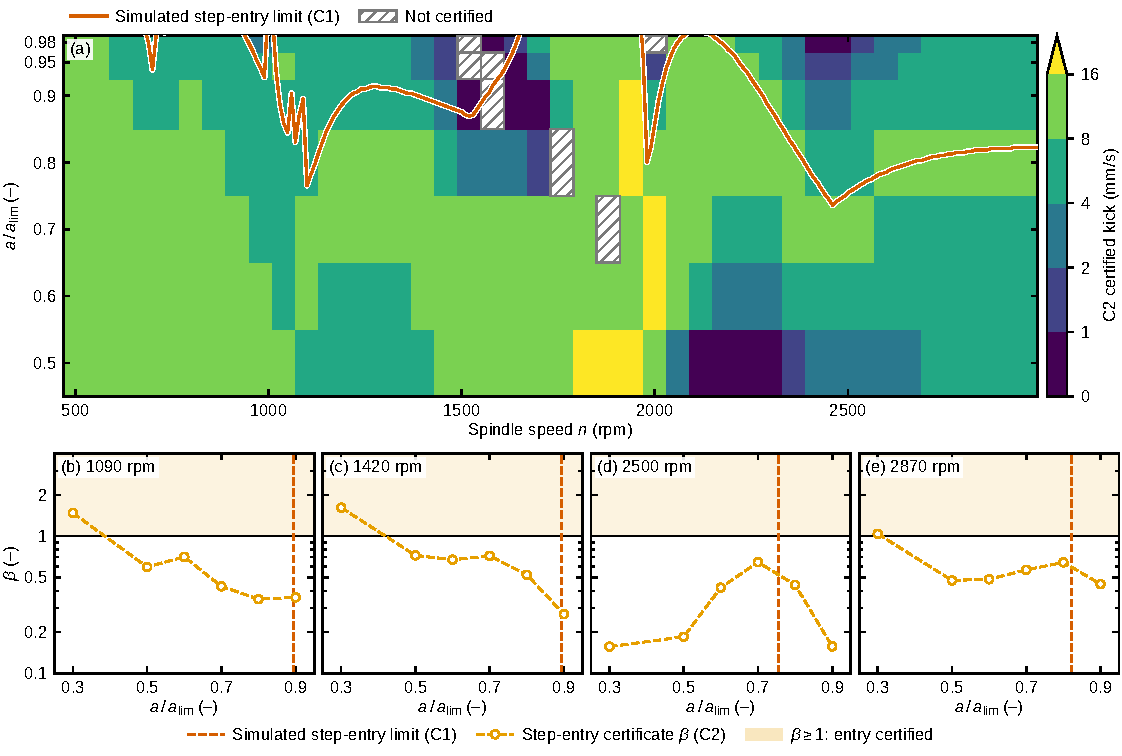
\includegraphics[width=\textwidth]{figures/fig07_certified_surface.pdf}
\caption{(a) Certified kick of the averaged model (C2) over spindle speed and depth on the gain map of Section~\ref{sec:feasibility}: 42 speeds, seven depths from 0.5 to $0.98\alim$; hatched: not certified (7 of 294 points); line: simulated step-entry limit of Section~\ref{sec:bistability}. (b)--(e) Step-entry certificate $\beta$ at the four speeds of Fig.~\ref{fig:cert}; $\beta\ge1$ (shaded) certifies the entry at rest on a fresh surface at the entry phase of the simulator; dashed: simulated step-entry limit. Command bound corrected as in Section~\ref{sec:cert-lmi}.}
\label{fig:surf}
\end{figure}

\subsection{Results on the periodic model (C3) and comparison with C2}\label{sec:cert-c3}

For the linear limit of this cutter averaging is nearly exact: on the gain map (126 speeds), the Floquet limit of the periodic collocated model is 0.99999--1.0011 times the averaged limit at half immersion and 0.99999--1.0028 times at the radial immersion $a_e/D=0.1$, never below it by more than $10^{-5}$ and without flip lobes (\ref{app:lmi}). The limits, 14--\SI{30}{\milli\metre} at half immersion and 30--\SI{65}{\milli\metre} at $a_e/D=0.1$, span one to five axial pitches $p_a$, over which the helix cancels most of the variation of $aH(t)$ \citep{insperger2006helix,zatarain2006helix}.
% src: README §14.4; results/c3_floquet.npz, c3_summary.json (floquet: 1.0000-1.0011 and 1.0000-1.0028, below_zoa 0, flip 0)

At the 48 points, 47 C3 certificates passed the check; at \SI{2500}{\rpm} and $0.98\alim$ none did (Table~\ref{tab:cert}). The ratio C3/C2 is 0.35--2.01 (median 1.064), and C3 exceeds C2 at 44 of the 47 points. The largest gains, 1.44--2.01, occur at \SI{2500}{\rpm} and 0.25--$0.5\alim$, where the worst segment leaves a margin of only 0.45--\SI{1.5}{\volt} and C2 is small (0.96--\SI{3.86}{\milli\metre\per\second}); at the other 40 points below $0.98\alim$ the ratio is 1.005--1.21. At $0.98\alim$, C3 falls below C2 (0.95, 0.98 and 0.35 at 1090, 1420 and \SI{2870}{\rpm}), although the critical kick of the periodic model there is not smaller than that of the averaged model: the loss is in the certificate, not in the basin. With 32 segments, C3 exceeds C2 at three of the four speeds (5.15, 2.31 and \SI{5.01}{\milli\metre\per\second} against 4.84, 2.08 and \SI{4.83}{\milli\metre\per\second}); \SI{2500}{\rpm} remains uncertified.
% src: README §14.5; results/c3_basin.npz (u0_min 1.143/0.593/0.451/1.487 V at 2500 rpm, 0.25-0.5 a_lim; periodic/averaged minimum kick at 0.98 a_lim 1.013/1.027/1.013/1.002), c3_edge.npz, c3_summary.json (basin, edge)

Phase by phase, the certificate lies below the simulated critical kick in all 448 cases (28 points with finite $\Delta v^*$, 16 phases) and below that of the periodic model in all 688 cases; none of the 3384 off-axis runs ended in chatter. From $0.7\alim$ upwards, $\Delta v^*/\beta$ is 1.46--4.78 (median 2.27) for C3 and 1.48--3.26 (median 2.35) for C2 at the same 18 points. The certificate varies by less than 3\,\% over the phases, except at \SI{2870}{\rpm} and $0.98\alim$ (1.70--\SI{2.01}{\milli\metre\per\second}): the optimisation maximises the worst phase and does not measure how the basin depends on the phase.
% src: README §14.5; results/c3_basin.npz (phase_cert spread <= 1.029 except 2870 rpm, 0.98 a_lim), c3_summary.json (basin: phase_cert_below_td 448/448, phase_cert_below_model 688/688, offaxis 0/3384, td_over_cert_from_07, td_over_c2_from_07)

The critical kick of the periodic model is 0.973--1.052 times that of the averaged model, phase by phase (704 pairs, median 1.001), and C2 lies below the critical kick of the periodic model at all 44 points where that kick is finite. The factor of about 2.3 between the certificates and the simulated basin near the limit is therefore not caused by averaging.
% src: README §14.5, §14.10; results/c3_summary.json (basin: periodic_over_averaged_model, c2_below_periodic_model 44/44)

At $0.9\alim$ and the four speeds, relative to C2, the periodic coefficient with the single level of C2 gives 0.94--0.98, the averaged model with the phase-dependent margin 1.06--1.15, and both together (C3) 1.02--1.12: the periodic model costs 2--6\,\%, and the phase-dependent margin gains 6--15\,\%. With a single level, a periodic $W$ cannot gain on the averaged model: the LMIs are linear in $(W,Y,S)$ and $\dot W$ integrates to zero over the period, so the period average of a feasible periodic certificate is a feasible constant one of the same size. The certificate is not converged in the number of segments: 8 give 0.93--1.03 and 32 give 1.08--1.22 (3--12\,\% above 16) at about twice the memory.
% src: README §14.6; results/c3_decomp.npz, c3_basin.npz, c3_summary.json (decomp)

At $a_e/D=0.1$, where $aH(t)$ varies more (over the four speeds 0.66--1.40 times its mean at $0.5\alim$ and 0.79--1.24 times at $0.9\alim$, against 0.77--1.27 and 0.88--1.11 at half immersion), all eight points (0.5 and $0.9\alim$) were certified, with C3/C2 = 0.94--1.04; the periodic and averaged critical kicks agree within 0.974--1.052, the certificate lies below $\Delta v^*$ in all 16 cases tested (four phases at the four points with finite $\Delta v^*$), and none of the 576 off-axis runs chattered.
% src: README §14.7; results/c3_lowimm.npz, c3_summary.json (lowimm); aH ranges re-evaluated in closed form (0.660-1.403, 0.787-1.241; 0.766-1.272, 0.881-1.109)

Averaging is known to fail in strongly interrupted cutting \citep{davies2002stability,bayly2003stability,merdol2004multi}. With straight teeth $aH(t)$ jumps as teeth enter and leave the cut, and at half immersion between 1600 and \SI{2100}{\rpm} (steps of \SI{25}{\rpm}) the uncontrolled cut has flip lobes below the averaged limit at 12 of 21 speeds (1675--\SI{1950}{\rpm}, from 0.947 of that limit). Where they persist with DVF ($g=\SI{100}{\volt\second\per\metre}$ at four speeds; the gain of the map at \SI{1950}{\rpm}), the forced orbit alone needs 27--\SI{66}{\volt} at 0.98 of the averaged limit, so $u_0<0$ and C2 claims nothing; gains of 250 and \SI{500}{\volt\second\per\metre} removed them, while gains of 141--\SI{250}{\volt\second\per\metre} and straight teeth at low immersion were not examined. Without control there is no forced command and the method of C2 does certify, which gives the counterexample of Table~\ref{tab:counter}: the averaged model, and with it the C2 certificate, is the same for both cutters, whereas the periodic model separates them. With straight teeth the cut is linearly unstable, though nearly benign in practice, its period-two oscillation staying at about \SI{1}{\micro\metre}.
% src: README §14.8 and the C3 summary at the head of the README; results/c3_straight.npz, c3_counter.npz (x_tooth alternation about 0.53 um, i.e. about 1 um peak to peak), c3_summary.json (straight, counter)

\begin{table}[!tbp]
\centering
\caption{Counterexample to averaging: \SI{1850}{\rpm}, no control ($g=0$), depth 0.98 times the averaged limit (\SI{23.6}{\milli\metre}), half immersion.}
\label{tab:counter}
\small
\begin{tabular}{@{}>{\raggedright\arraybackslash}p{0.34\textwidth}>{\raggedright\arraybackslash}p{0.29\textwidth}>{\raggedright\arraybackslash}p{0.27\textwidth}@{}}
\toprule
 & Straight teeth & Helical teeth (\ang{45})\\
\midrule
Critical Floquet multiplier & $\lvert\mu\rvert=1.034$ at \ang{180} & $\lvert\mu\rvert=0.977$ at \ang{177}\\
C2 certificate (averaged model) & \SI{13.2}{\milli\metre\per\second} & \SI{13.2}{\milli\metre\per\second}\\
C3 certificate (periodic model) & none (linearly unstable) & \SI{13.1}{\milli\metre\per\second}\\
Simulator after a \SI{0.1}{\milli\metre\per\second} kick & never settles; period-two oscillation of about \SI{1}{\micro\metre} & settles\\
\bottomrule
\end{tabular}
\end{table}
% src: README §14.8; results/c3_counter.npz (a 23.63 mm, mu_abs 1.0342/0.9767, mu_arg 180/177 deg, c2_size 13.201, c3_size 0/13.090 mm/s, sim_stable False/True), log_c3_counter.txt

\subsection{Limitations}\label{sec:cert-limits}

The certificates are theorems about $N$-node collocations of the averaged (C2) and the time-periodic (C3) model, not about the delay equation, which would need a Lyapunov--Krasovskii functional \citep{seuret2014bessel}, nor about the simulator. The chip vanishing near the exit angle is outside both models, the validity bound ($\delta=0.5$, a choice) excludes only gross loss of contact, and no decay rate is claimed. The step-entry certificate covers one entry phase, does not reach productive depths and was not computed on the periodic model, which would need a phase-dependent condition. The periodic certificate is not converged in the number of segments. The forced command of the simulator, computed with 30 axial layers, exceeds the closed form of the certificates by up to 8.7\,\% at the operating points of Section~\ref{sec:feasibility}, so the simulator's margin is slightly narrower; no comparison above changes, as every certificate lies below the simulated basin. The model has one mode, and nothing was tested experimentally.
% src: README §12.7 (limits), §14.10 (limits), §3 (cf_vs_td_layers: up to +8.7 %)
